\documentclass[8pt]{beamer}

\usepackage[french]{babel}
\usepackage[OT1]{fontenc}
\usepackage[utf8]{inputenc}
\usepackage{tcolorbox}
\usepackage{listings}
\usepackage{caption}
\usepackage{amsthm}

\usetheme{Antibes}
\graphicspath{{imgs_oral/}}

\definecolor{darkWhite}{rgb}{0.94,0.94,0.94}
\definecolor{darkGreen}{rgb}{0.2,0.5,0.2}
\definecolor{lightYellow}{rgb}{0.7,0.55,0.2}
 
\lstset{
    backgroundcolor=\color{darkWhite},
    breakatwhitespace=false,
    breaklines=true,
    captionpos=b,
    commentstyle=\color{darkGreen},
    deletekeywords={void},
    escapeinside={\%*}{*)},
    extendedchars=true,
    keepspaces=true,
    keywordstyle=\color{cyan},
    language=C,
    morekeywords={__m256i, Uint},
    showspaces=false,
    showstringspaces=false,
    showtabs=false,
    stepnumber=1,
    stringstyle=\color{gray},
    tabsize=2,
    title=\lstname,
} 

\lstdefinestyle{frameStyle}{
    basicstyle=\footnotesize,
    numbers=left,
    numbersep=20pt,
    numberstyle=\tiny\color{black}
}

\captionsetup[table]{name=Tableau}

\title{Implémentations efficaces de calculs sur les polynômes à une variable : FFT}
\author{Pierre Lin, Enzo Roaldes}
\institute{L2 DM-IM 2022, Sorbonne Université}
\date{13 Juillet 2022}
\titlegraphic{
\includegraphics[scale=0.22]{./logo}}

\expandafter\def\expandafter\insertshorttitle\expandafter{%
  \insertshorttitle\hfill%
  \insertframenumber\,/\,\inserttotalframenumber}

\begin{document}

\frame{\titlepage}


\begin{frame}
\frametitle{Introduction}

Les polynômes sont :
\begin{itemize}
    \item un objet mathématique fondamental
    \item omniprésents dans notre quotidien \newline
\end{itemize}

Plan de la soutenance :
\begin{itemize}
    \item Algorithme Naïf \& de Karatsuba
    \item Fast Fourier Transform (FFT)
    \item Vectorisation avec AVX2 \newline
\end{itemize}

Langage utilisé : C

\end{frame}


\begin{frame}
\frametitle{Algorithme Naïf}

Les polynômes sont représentés par des tableaux contenant leurs coefficients. \\[0.2cm]


L'algorithme naïf est basé sur la formule :
\[R(X) = PQ(X) =
\displaystyle\sum_{i=0}^{n}\sum_{j=0}^{n} p_i q_j X^{i+j}\]
\\[0.4cm]
Complexité = nombre d'opérations élémentaires.\\[0.4cm]
Complexité de l'algorithme naïf : $O(n^2)$


\end{frame}


\begin{frame}
\frametitle{Algorithme de Karatsuba}

Principe de l'algorithme de Karatsuba :
\begin{itemize}
    \item Décomposition récursive de P et Q : \\
    $P = P_1 + X^{n/2}P_2$ $Q = Q_1 + X^{n/2}Q_2$
    \item Reconstruction du résultat R :
    $R = E_1+X^{n/2}(E_3-E_2-E_1)+X^n E_2$\\
    avec $E_1 = P_1Q_1\ ; E_2 = P_2Q_2\ et\ E_3 = (P_1+P_2)(Q_1+Q_2)$
\end{itemize}
\ \\[0.2cm]
Complexité : $O(n^{1.58})$ \\[0.5cm]

\begin{center}
\begin{tabular}{||c c c||}
\hline
Degré de $P$ et $Q$ & Naïf & Karatsuba \\
\hline\hline
$2^{15}$ & 0.429183 & 0.085549 \\
\hline
$2^{16}$ & 1.761229 & 0.242966 \\
\hline
$2^{17}$ & 6.875559 & 0.645986 \\
\hline
$2^{18}$ & 28.165627 & 2.023236 \\
\hline
\end{tabular}
\end{center}
{\captionof{table}{Temps de l'algorithme naïf et de l'algorithme de Karatsuba.}}
\end{frame}

\begin{frame}
\frametitle{Quelques notions fondamentales}

\begin{enumerate}
    \only<1, 2, 3, 4, 5>{\item $n = 2^k$ sera le degré du polynôme final $R = PQ$ \newline}
    \only<2, 3, 4, 5>{\item Le corps $\mathbb{Z}/p\mathbb{Z}$ \newline}
    \only<3, 4, 5>{\item Racine primitive $p-1$-ième de l'unité $r$ : $r^{p-1}\ \%\ p = 1$ et que $r^{k}\ \%\ p \ne 1$\\[0.1cm] pour tout $k$ dans $\{1,\dots,p-2\}$\newline} 
    \only<4, 5>{\item Racine principale $n$-ième de l'unité : $r\_principale = r^\frac{p-1}{n}\ \% \ p$ 
    \\[0.1cm] $\Rightarrow p-1$ doit être divisible par $n$\newline} 
    \only<5>{\item Choix du nombre premier $p = 754974721 = 1+2^{24}*3^2*5$\\[0.1cm]
    $\Rightarrow deg_{max}(R) = 2^{24}$ \\[0.1cm]
    racine primitive $p-1$-ième de l'unité : $r = 11$}
    
\end{enumerate}

\end{frame}


\begin{frame}
\frametitle{Algorithme de multiplication par FFT}
\newtheorem{Thm1}{Théorème \textit{(Interpolation de Lagrange)}}
\begin{Thm1}
Soient $a_1,\dots,a_n$ et $b_1,\dots,b_n$ dans $\mathbb{Z}/p\mathbb{Z}$  (avec les $a_i$ deux à deux distincts). Alors il existe un unique polynôme P de degré $< n$ tel que :
\begin{center}
$\forall i \in \{1,..., n\},\ P(a_i)\ =\ b_i$.
\end{center}
\end{Thm1}

\begin{tcolorbox}[colback=cyan!5!white,
                  colframe=cyan!100!black,
                  title=\textbf{Algorithme de multiplication par FFT}
                 ]
\textbf{Entrée.} $P$ et $Q$ deux polynômes, $n$ une puissance de $2$ avec $n>deg(PQ)$ et $\omega$ une racine principale $n$-ième de l’unité. \\[0.1cm]
\textbf{Sortie.} $R = PQ$ \\[0.1cm]
\textbf{Algorithme.} \\[0.1cm]
1. \textit{Pré-calcul}. Calculer les puissances $\omega^0,\omega^1,\omega^2,\dots,\omega^{n-1}$ $\to$ $O(n)$ \\[0.2cm]
2. \textit{Évaluation (DFT)}. Calculer les valeurs : \\[0.1cm] $Eval(P)=(P(\omega^0),\dots,P(\omega^{n-1}))$ ; $Eval(Q)=(Q(\omega^0),\dots,Q(\omega^{n-1}))$. \\[0.2cm]
3. \textit{Produit point à point}. $Eval(R) = (PQ(\omega^0),\dots,PQ(\omega^{n-1}))$ $\to$ $O(n)$ \\[0.2cm]
4. \textit{Interpolation}. Retrouver $R$ grâce à $Eval(R)$.
\end{tcolorbox}

\end{frame}

\begin{frame}
\frametitle{Discrete Fourier Transform (DFT)}

\underline{Principe de la DFT (diviser pour régner)} : \\[0.3cm]
Soient $n = 2^k$ et $P(X) = p_n X^n +\dots+p_1 X + p_0$. \\[0.2cm]
Soient $P_0$, $P_1$ les polynômes composés des coefficients de rang respectivement pair et impair de $P$ : \\
$P_0(X) = p_{n} X^{n/2} +\dots+ p_2 X + p_0\ et\ P_1(X) = p_{n-1} X^{(n-2)/2} +\dots+ p_3 X + p_1$. \\[0.2cm]
Nous avons alors que $P(X) = P_0(X^2)+X P_1(X^2)$. \\[0.1cm]
$\to$ Algorithme récursif où nous divisons $n$ par $2$

\end{frame}

\begin{frame}
\frametitle{DFT}

\begin{tcolorbox}[colback=cyan!5!white,
                  colframe=cyan!100!black,
                  title=\textbf{Algorithme DFT}
                 ]
\textbf{Entrée.} $P = p_0+\dots+p_{n-1}X^{n-1}$, $n$ une puissance de $2$ et le tableau $ racines = [1, \omega,\dots,\omega^{n-1}]$ où $\omega$ est une racine $n$-ième principale de l'unité.\\[0.1cm]
\textbf{Sortie.} $P(1),\dots,P(\omega^{n-1})$.\\[0.1cm]
\textbf{Algorithme.} \\[0.1cm]
1. \textit{}Si $n=1$, renvoyer $p_0$. \\ [0.1cm]
2. \textit{}Sinon, soit $k=n/2$. Calculer :\\
\[ R_0(X) = \sum_{i=0}^{k-1}(p_i+p_{i+k})X^i \]
\[ R_1(X) = \sum_{i=0}^{k-1}(p_i-p_{i+k})\omega^iX^i \]
3. \textit{}Calculer récursivement $R_0(1), R_0(\omega^2),\dots,R_0((\omega^2)^{k-1})$ \\ [0.1cm]
et $R_1(1), R_1(\omega^2),\dots,R_1((\omega^2)^{k-1})$. \\[0.2cm]
4. \textit{}Renvoyer $R_0(1), R_1(1), R_0(\omega^2), R_1(\omega^2),\dots, R_0((\omega^2)^{k-1}), R_1((\omega^2)^{k-1})$.
\end{tcolorbox}
\ \\

\end{frame}

\begin{frame}
\frametitle{Opérations modulo $p$}

Opération \% beaucoup plus lente que les opérations $+$, $-$, $*$. \\[0.5cm]
Addition modulo $p$ :
\[ (a+b)\ \%\ p = 
\left\{\begin{array}{@{}l@{}}
a + b - p\ \ \ \ \ si\ a+b \geq p\\
a + b\ \ \ \ \ \ \ \ \ \ sinon
\end{array}\right.\,\ \] \\
Soustraction modulo $p$ :
\[ (a-b)\ \%\ p = 
\left\{\begin{array}{@{}l@{}}
p - (b - a)\ \ \ \ \ si\ b > a\\
a - b\ \ \ \ \ \ \ \ \ \ \ \ sinon
\end{array}\right.\,\]\\[0.2cm]

Multiplication modulo $p$ : cast en $long$ puis utilisation de l'opérateur \%.

\end{frame}

\begin{frame}
\frametitle{Première version DFT}

Malloc des tableaux $R_0$, $R_1$ et $racines$ à chaque récursion.\\[0.3cm]

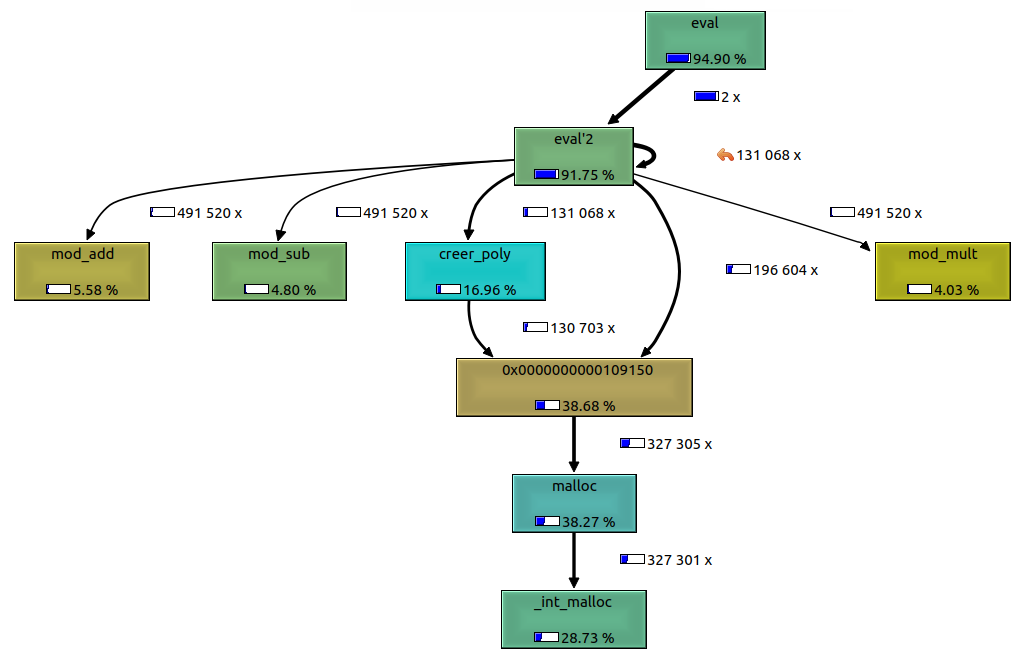
\includegraphics[scale=0.5]{profiler_eval_malloc.png}

$\to$ Utilisation d'un $pas$ pour le tableau $racines$.\\ 
$\to$ Utilisation du tableau des coefficients de $P$ pour $R_0$ et $R_1$.

\end{frame}

\begin{frame}
\frametitle{DFT}

\begin{tcolorbox}[colback=cyan!5!white,
                  colframe=cyan!100!black,
                  title=\textbf{Algorithme DFT}
                 ]
\textbf{Entrée.} $P = p_0+\dots+p_{n-1}X^{n-1}$, $n$ une puissance de $2$ et le tableau $ racines = [1, \omega,\dots,\omega^{n-1}]$ où $\omega$ est une racine $n$-ième principale de l'unité.\\[0.1cm]
\textbf{Sortie.} $P(1),\dots,P(\omega^{n-1})$.\\[0.1cm]
\textbf{Algorithme.} \\[0.1cm]
1. \textit{}Si $n=1$, renvoyer $p_0$. \\ [0.1cm]
2. \textit{}Sinon, soit $k=n/2$. Calculer :\\
\[ R_0(X) = \sum_{i=0}^{k-1}(p_i+p_{i+k})X^i \]
\[ R_1(X) = \sum_{i=0}^{k-1}(p_i-p_{i+k})\omega^iX^i \]
3. \textit{}Calculer récursivement $R_0(1), R_0(\omega^2),\dots,R_0((\omega^2)^{k-1})$ \\ [0.1cm]
et $R_1(1), R_1(\omega^2),\dots,R_1((\omega^2)^{k-1})$. \\[0.2cm]
4. \textit{}Renvoyer $R_0(1), R_1(1), R_0(\omega^2), R_1(\omega^2),\dots, R_0((\omega^2)^{k-1}), R_1((\omega^2)^{k-1})$.
\end{tcolorbox}
\ \\

\end{frame}

\begin{frame}[fragile]
\frametitle{AVX2}

Vectorisation avec AVX2 :\\[0.2cm]
\begin{itemize}
    \item opérations élémentaires ($+$, $-$, $*$, ...) sur des "vecteurs" de données similaires à des tableaux.
    \item type $\_\_mm256i$ : stock 256 bits d'entiers $\to$ stockage de 8 entiers de 32 bits.
    \item opérations sur deux $\_\_mm256i$ aussi rapide que sur deux entiers $int$.\\ $\to$ possibilité d'un gain de temps fois $8$ en utilisant AVX2.
\end{itemize}
\ \\[0.2cm]
\textit{Exemple :} 
\begin{lstlisting}
__m256i a = _mm256_set_epi32(1, 2, 3, 4, 5, 6, 7, 8);
__m256i b = _mm256_set_epi32(1, 0, 1, 0, 1, 0, 1, 0);
__m256i x = _mm256_add_epi32(a, b);
// nous avons x = [2, 2, 4, 4, 6, 6, 8, 8]
\end{lstlisting}
\end{frame}

\newtheorem{Ex1}{Comment faire le modulo sur des vecteurs ?}
\newtheorem{Ex2}{Exemple}
\newtheorem{Ex3}{Preuve}


\begin{frame}
\frametitle{Opérations modulo $p$ avec AVX2}
Pas d'opération modulo en AVX2 !
\only<1, 2>{
\begin{Ex1}
Soient $p = 7, \ \overrightarrow{a} = [6, 2], \ \space \overrightarrow{b} = [4, 1]$ \ et $ \ \overrightarrow{x} = \overrightarrow{a}+\overrightarrow{b} = [10, 3]$.  \textbf{\textcolor{red}{Problème} !}
\end{Ex1}}
 
\only<2>{$\to$ Fonction AVX2 $\_mm256\_min\_epu32(\overrightarrow{a}, \overrightarrow{b})$ : permet de prendre le minimum "positif" entre chaque élément de $\overrightarrow{a}$ et $\overrightarrow{b}$.

\begin{Ex2} 
$min\_pos([1, 4],\  [0, -10]) = min([1, 4], \ [0,$ UINT\_MAX$-10]) = [0, 4]$.
\end{Ex2}

\indent Pour l'addition, avec $\overrightarrow{x} = \overrightarrow{a}+\overrightarrow{b}$, on a $\overrightarrow{x}\ \%\ \overrightarrow{p} = min\_pos(\overrightarrow{x}, \overrightarrow{x}-\overrightarrow{p})$.

\begin{Ex3}
Si $\overrightarrow{x}[i] \geq p$, alors l'appel retourne $\overrightarrow{x}[i] - p$. \\[0.2cm]
Sinon, $\overrightarrow{x}[i] < p$, donc $\overrightarrow{x}[i]-p < 0$, et après conversion en $Uint$ : \\
$\overrightarrow{x}[i]-p > \overrightarrow{x}[i]$
et donc l'appel retourne $\overrightarrow{x}[i]$.
\end{Ex3}

De même, pour la soustraction, avec $\overrightarrow{x} = \overrightarrow{a}-\overrightarrow{b}$, on a : 
$\overrightarrow{x}\ \%\ \overrightarrow{p} = min\_pos(\overrightarrow{x}, \overrightarrow{x}+\overrightarrow{p})$.}

\end{frame}


\begin{frame}[fragile]
\frametitle{Opérations modulo $p$ avec AVX2}

\begin{lstlisting}
void vect_mod_add(Uint *res1, Uint *tab1, Uint *tab2) {
    __m256i p = _mm256_set1_epi32(NB_P);
    __m256i a = _mm256_loadu_si256((__m256i *) tab1);
    __m256i b = _mm256_loadu_si256((__m256i *) tab2);
    __m256i x = _mm256_add_epi32(a, b);
    __m256i result = _mm256_min_epu32(x, _mm256_sub_epi32(x, p));
    _mm256_storeu_si256((__m256i *) res1, result);
}
\end{lstlisting}

Multiplication : Algorithme de réduction de Barrett

\begin{center}
\begin{tabular}{||c c c||}
\hline
Opération & Sans AVX2 & Avec AVX2 \\
\hline\hline
Addition & 0.012610 & 0.006697 \\
\hline
Soustraction & 0.014247 & 0.007139 \\
\hline
Multiplication & 0.015053 & 0.007497 \\
\hline
\end{tabular}
\end{center}
{\captionof{table}{Temps des opérations d'addition, soustraction et multiplication sans et avec AVX2.}}

\end{frame}

\begin{frame}
\frametitle{DFT}

\begin{tcolorbox}[colback=cyan!5!white,
                  colframe=cyan!100!black,
                  title=\textbf{Algorithme DFT}
                 ]
\textbf{Entrée.} $P = p_0+\dots+p_{n-1}X^{n-1}$, $n$ une puissance de $2$ et le tableau $ racines = [1, \omega,\dots,\omega^{n-1}]$ où $\omega$ est une racine $n$-ième principale de l'unité.\\[0.1cm]
\textbf{Sortie.} $P(1),\dots,P(\omega^{n-1})$.\\[0.1cm]
\textbf{Algorithme.} \\[0.1cm]
1. \textit{}Si $n=1$, renvoyer $p_0$. \\ [0.1cm]
2. \textit{}Sinon, soit $k=n/2$. Calculer :\\
\[ R_0(X) = \sum_{i=0}^{k-1}(p_i+p_{i+k})X^i \]
\[ R_1(X) = \sum_{i=0}^{k-1}(p_i-p_{i+k})\omega^iX^i \]
3. \textit{}Calculer récursivement $R_0(1), R_0(\omega^2),\dots,R_0((\omega^2)^{k-1})$ \\ [0.1cm]
et $R_1(1), R_1(\omega^2),\dots,R_1((\omega^2)^{k-1})$. \\[0.2cm]
4. \textit{}Renvoyer $R_0(1), R_1(1), R_0(\omega^2), R_1(\omega^2),\dots, R_0((\omega^2)^{k-1}), R_1((\omega^2)^{k-1})$.
\end{tcolorbox}
\ \\

\end{frame}

\newtheorem{Preuve1}{Preuve que $u$ est l'inverse de $a$}
\newtheorem{ThmBezout}{Théorème de Bézout}
\begin{frame}
\frametitle{Suite de la multiplication par FFT}
L'étape d'interpolation dans la multiplication par FFT :
\begin{enumerate}
    \item Calculer les puissances successives de l'inverse de la racine principale : \\
   $\omega^{0},\omega^{-1},\omega^{-2},\dots,\omega^{-(n-1)}$.
    \item Appliquer la DFT à $Eval(R)$ avec ces inverses.
    \item Diviser les coefficients obtenus suite à la DFT par $n$ (c'est-à-dire multiplier par l'inverse de $n$ dans $\mathbb{Z}/p\mathbb{Z}$).
\end{enumerate}
\ \\[0.2cm]
Comment calculer $\omega^{-1}$ et $n^{-1}$ dans $\mathbb{Z}/p\mathbb{Z}$? \\[0.1cm]
$\to$ Algorithme d'Euclide étendu appliqué à l'équation $au+pv=1$.

\begin{ThmBezout}
Soient $a$ et $b$ deux entiers naturels non nuls. a et b sont premiers entre eux si et seulement si il existe deux entiers relatifs $u$ et $v$ tels que $au + bv = 1$.
\end{ThmBezout}

\begin{Preuve1}
\begin{enumerate}
    \item $a$ et $p$ sont premiers entre eux donc $\exists u,v \in \mathbb{Z}$ tels que $au + pv = 1$
    \item Si $au+pv=1$, alors dans $\mathbb{Z}/p\mathbb{Z}$ : \newline
    $au+pv = (au+pv)\%p = (au)\%p + (pv)\%p = (au)\%p = 1$.
    \item Donc $au=1$ dans $\mathbb{Z}/p\mathbb{Z}$ et $u$ est l'inverse de $a$ dans $\mathbb{Z}/p\mathbb{Z}$.
\end{enumerate} 
\end{Preuve1}
\end{frame}

\begin{frame}
\frametitle{Améliorations}

\begin{center}
\begin{tabular}{||c c c||}
\hline
$n$ & FFT Sans AVX2 & FFT Avec AVX2 \\
\hline\hline
$2^{20}$ & 0.158404 & 0.150727 \\
\hline
$2^{21}$ & 0.503089 & 0.437402 \\
\hline
$2^{22}$ & 1.240285 & 1.075995 \\
\hline
$2^{23}$ & 3.028623 & 2.317684 \\
\hline
$2^{24}$ & 7.108149 & 5.847869 \\
\hline
\end{tabular}
\end{center}
\ \\[0.2cm]

Rechercher les cases désirées dans $racines$ avec AVX2 prend trop de temps.\\
\begin{itemize}
    \item Réutilisation du $malloc$ pour le tableau $racines$.\\[0.2cm]
    \item Gain de temps sur les polynômes de degré $> 20$.\\[0.2cm]
\end{itemize}
\ \\[0.2cm]

\begin{center}
\begin{tabular}{||c c c||}
\hline
$n$ & FFT Sans AVX2 & FFT Avec AVX2 (Version 2) \\
\hline\hline
$2^{20}$ & 0.158404 & 0.180472 \\
\hline
$2^{21}$ & 0.503089 & 0.355293 \\
\hline
$2^{22}$ & 1.240285 & 0.706925 \\
\hline
$2^{23}$ & 3.028623 & 1.504402 \\
\hline
$2^{24}$ & 7.108149 & 2.939824 \\
\hline
\end{tabular}
\end{center}


\end{frame}

\begin{frame}
\frametitle{La bibliothèque NTL}

Meilleure bibliothèque pour la FFT dans $\mathbb{Z}/p\mathbb{Z}$ : NTL\\[0.3cm]

Comparaison des temps obtenus : \\[0.3cm]

\begin{center}
\begin{tabular}{||c c c c c||}
\hline
$n$ & No AVX2 (NTL) & No AVX2 & AVX2 (NTL) & AVX2 \\
\hline\hline
$2^{18}$ & 0.00297 & 0.01017 & 0.00182 & 0.00944 \\
\hline
$2^{20}$ & 0.01517 & 0.06008 & 0.01113 & 0.06168 \\
\hline
$2^{22}$ & 0.08613 & 0.38058 & 0.07253 & 0.21169 \\
\hline
\end{tabular}
\end{center}
\ \\[0.3cm]
NTL est 3 à 5 fois plus rapide que nous !

\end{frame}

\begin{frame}
\frametitle{Temps finaux et Conclusion}

\begin{center}
\begin{tabular}{||c c c c c||}
\hline
$n$ & Naïf & Karatsuba & FFT Sans AVX2 & FFT Avec AVX2 V2 \\
\hline\hline
$2^{18}$ & 28.17 & 2.02 & 0.037 & 0.045 \\
\hline
$2^{19}$ & 2 m & 6.07 & 0.085 & 0.094 \\
\hline
$2^{20}$ & 7.5 m & 18.21 & 0.16 & 0.18 \\
\hline
$2^{21}$ & 30 m & 54.63 & 0.50 & 0.36 \\
\hline
$2^{22}$ & 2 h & 2.7 m & 1.24 & 0.71 \\
\hline
$2^{23}$ & 8 h & 8.1 m & 3.03 & 1.50 \\
\hline
$2^{24}$ & \textbf{\textcolor{red}{32 h}} & 24.5 m & 7.11 & \textbf{\textcolor{red}{2.94}} \\
\hline
\end{tabular}
\end{center}
{\captionof{table}{Comparaison finale des algorithmes implémentés}}

Attention ! Le degré des polynômes multipliés par FFT est limité par le choix de $p$.\\
D'un autre côté : Karatsuba et Naïf peuvent multiplier n'importe quoi !\\[0.2cm]

Temps de nos algorithmes $\approx 5$ fois le temps sur NTL \\[0.2cm]
Algorithmes plus performants d'ici là ? Dépassé par de nouvelles technologies ?\\[0.2cm]

\end{frame}

\end{document}